\documentclass[12pt]{article}
\usepackage[margin=1in]{geometry} 
\usepackage[shortlabels]{enumitem}
\usepackage{caption}
\usepackage{algorithm}
\usepackage[noend]{algpseudocode}
\usepackage[table,xcdraw]{xcolor}
\usepackage{import}
\usepackage{tikz}
\usepackage{tikz,fullpage}
\usetikzlibrary{arrows, automata}
\usepackage{tkz-berge}
\usepackage[position=top]{subfig}
\usepackage{amsmath,amsthm,amssymb,amsfonts, enumitem, fancyhdr, color, comment, graphicx, environ}
\pagestyle{fancy}
\setlength{\headheight}{65pt}
\newenvironment{problem}[2][Problem]{\begin{trivlist}
\item[\hskip \labelsep {\bfseries #1}\hskip \labelsep {\bfseries #2.}]}{\end{trivlist}}
\newenvironment{sol}
    {\emph{Solution:}
    }
    {
    \qed
    }
\specialcomment{com}{ \color{blue} \textbf{Comment:} }{\color{black}} %for instructor comments while grading
\NewEnviron{probscore}{\marginpar{ \color{blue} \tiny Problem Score: \BODY \color{black} }}
% creates keywords for input and output in algorithm block
\algblock{Input}{EndInput}
\algnotext{EndInput}
\algblock{Output}{EndOutput}
\algnotext{EndOutput}
\newcommand{\Desc}[2]{\State \makebox[13em][l]{#1}#2}
\lhead{Mazen Alotaibi \textit{(alotaima)}}
\rhead{CS 420 \\ Section 001 \\ Winter 2019 \\ HW 4}

\begin{document}

\Procedure{reachability}{}
\State $sortedList = Sort(v)$ 
\State $visited = \empty$
\For{\textbf{$v_i$}  \textbf{ $\in$ } $sortedList$}
    \If {$v_i\ \not \in visited$}
        \State $min = BFS(v)$
        \State $visited.append(BFS(v))$
    \EndIf
\EndFor
\EndProcedure
\Procedure{HK}{$G$, $n$}
    \For{$k$ \textbf{from} $2$ \textbf{to} $n$}
        \State $C(\{k\},k)=d_{1, k}$
    \EndFor
    \For{$s$ \textbf{from} $2$ \textbf{to} $n-1$}
        \For{$all\ S \subseteq \{2,...,n\}, |S|=s$}
            \For{$all\ k \in S$}
                \State $\{C(S,k)=min_{m \neq k, m \in S}[C(S-\{k\},m)+d_{m, k}]\}$
            \EndFor
        \EndFor
    \EndFor
    \State $opt=min_{k \neq 1}[C(\{2, 3, ..., n\}, k) + d_{k, 1}]$
    \State \textbf{return} $opt$
\EndProcedure
\begin{problem}{3: Food Truck Orders.} The Acme food truck produces a large variety of different...
\end{problem}
\begin{sol}
This problem is a max flow problem. By using Ford-Fulkerson algorithm, the result of the algorithm is a set of food assignments. The maximum number of happy customers means the minimum number of vouchers. The time complexity is $O(mn^2)$ as the number of edges is $E=mn$ and the max flow $|f|\leq n$.
\end{sol}
\newpage

\begin{figure}[h]
\begin {center}
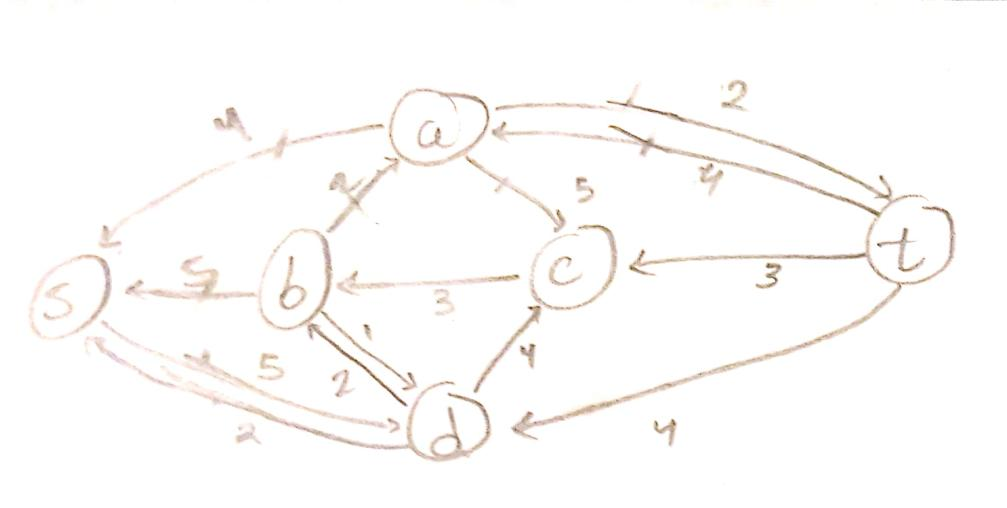
\includegraphics[width=\textwidth]{fig/1.jpg}
\caption*{Graph 1: the residual network $G_f$}
\end{center}
\centering
\end{figure}

\begin{figure}[h]
\begin {center}
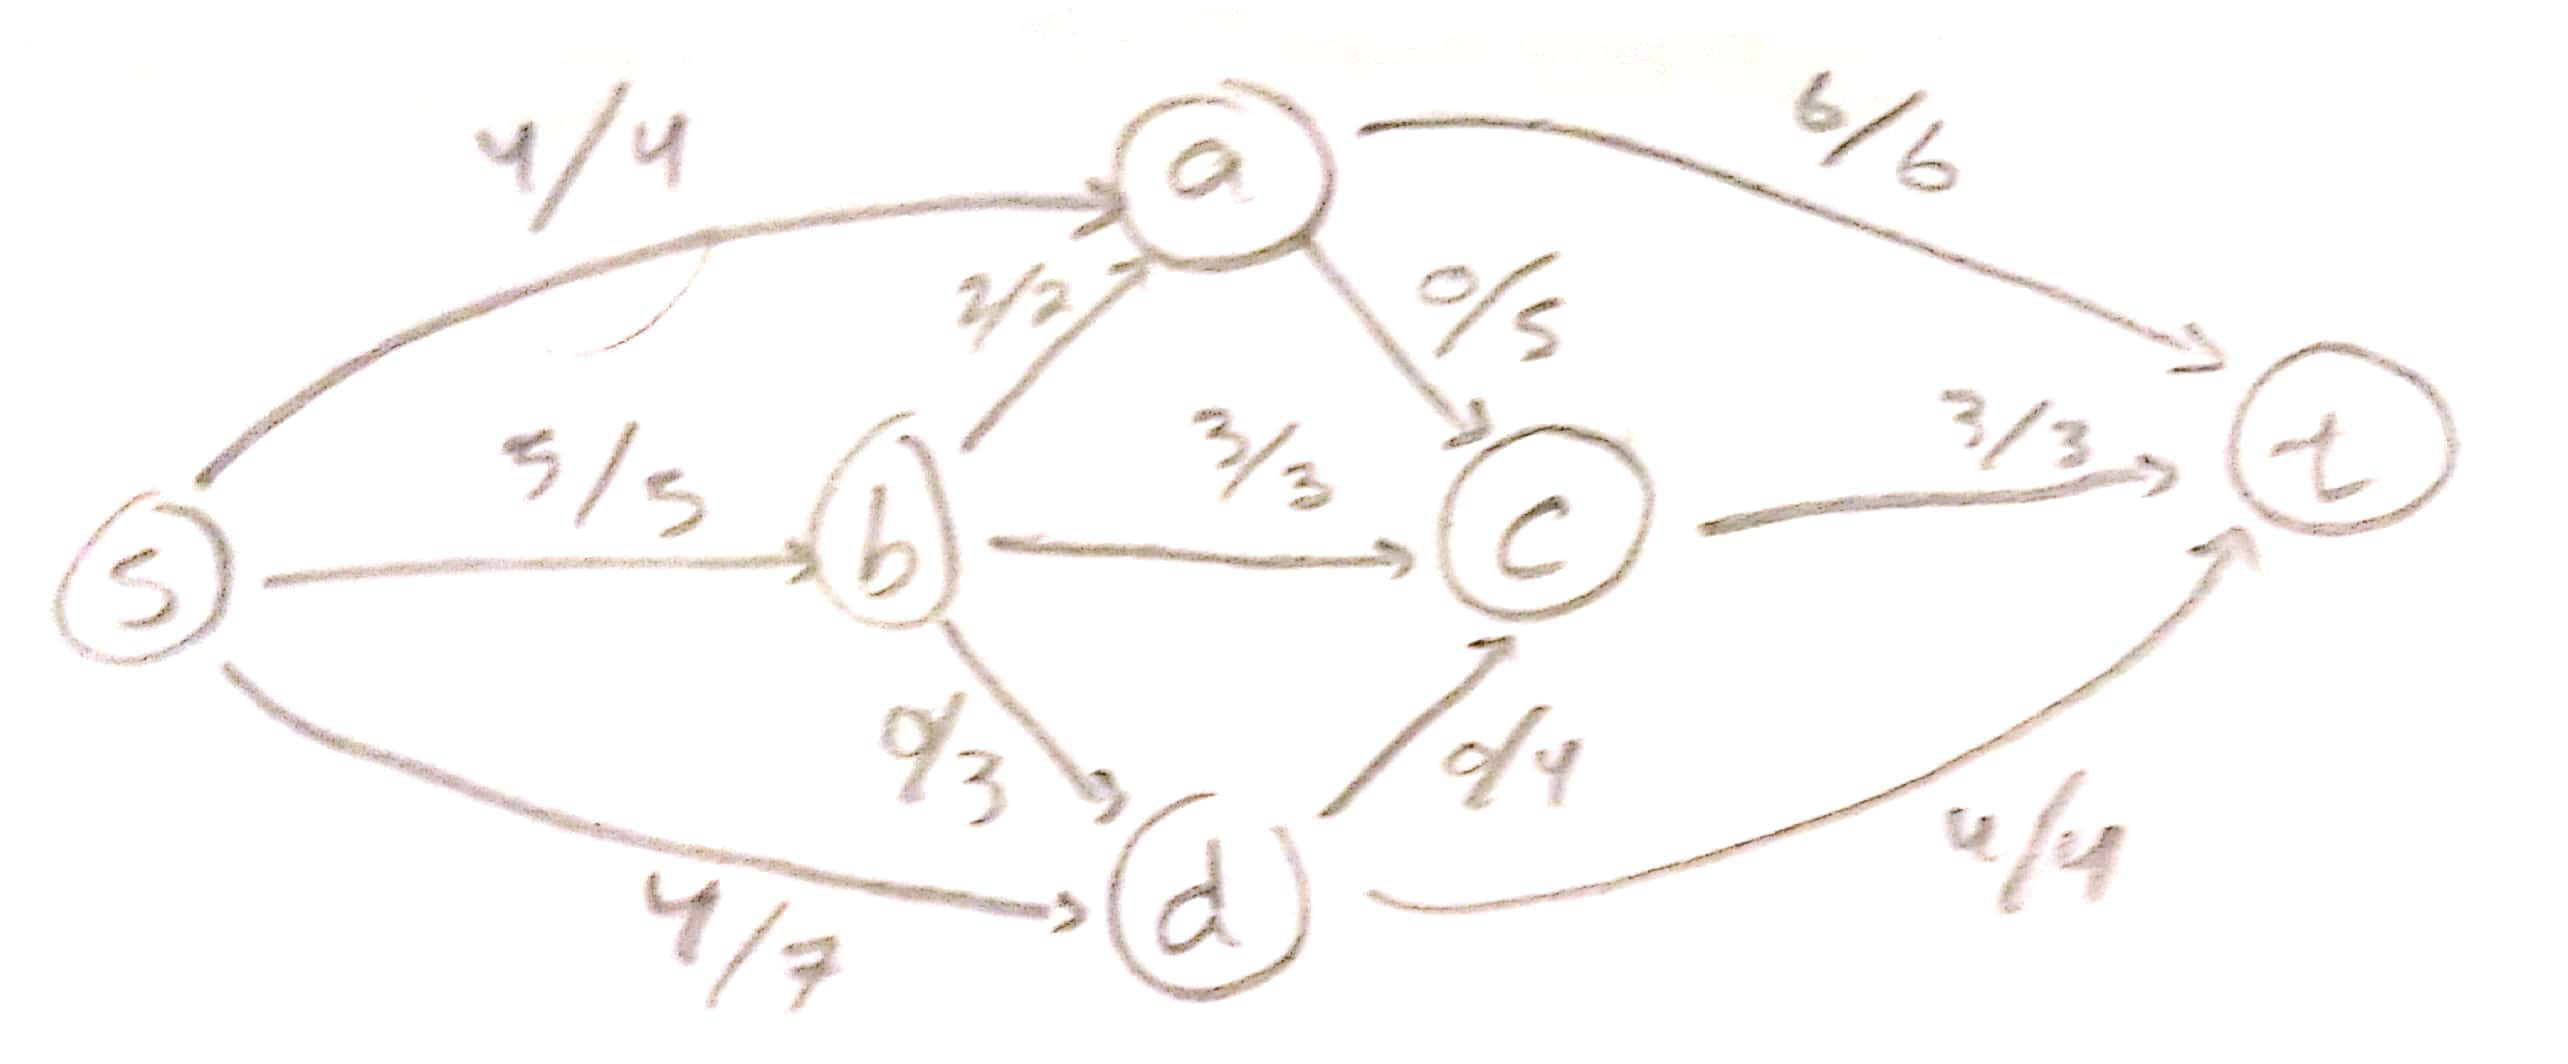
\includegraphics[width=\textwidth]{fig/2.jpg}
\caption*{Graph 2: the updated flow}
\end{center}
\centering
\end{figure}

\begin{figure}[h]
\begin {center}
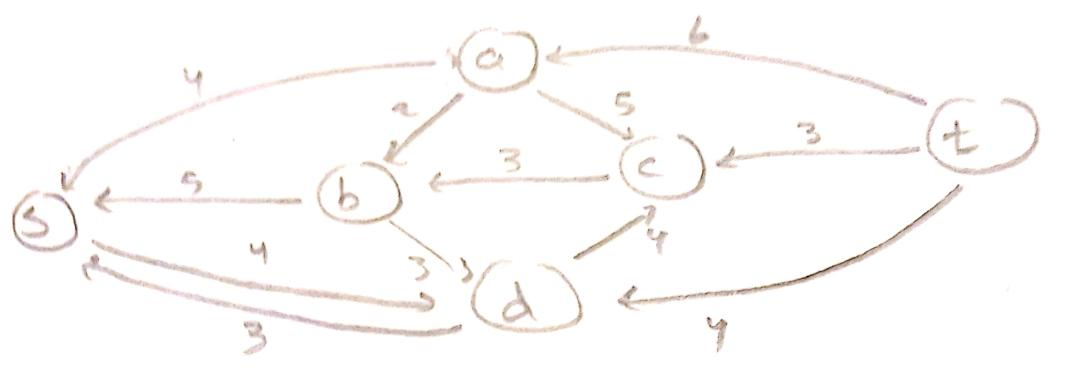
\includegraphics[width=\textwidth]{fig/3.jpg}
\caption*{Graph 3: the updated residual network}
\end{center}
\centering
\end{figure}

\begin{figure}[h]
\begin {center}
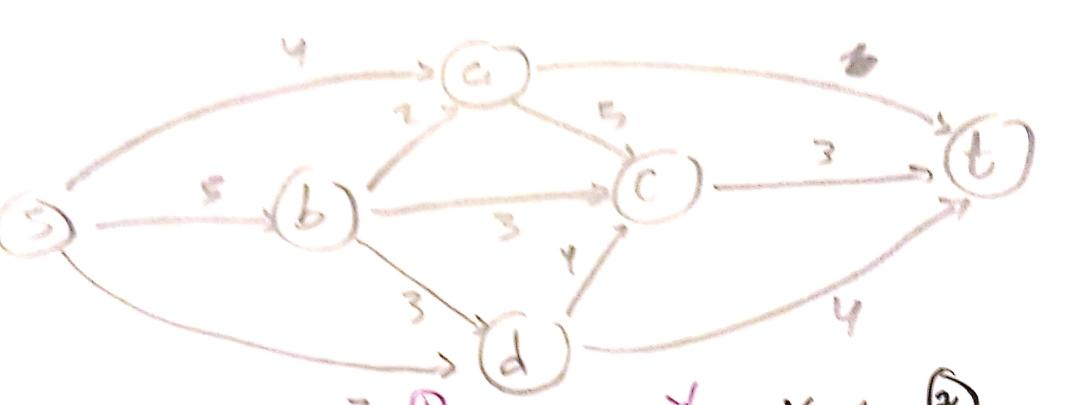
\includegraphics[width=\textwidth]{fig/4.jpg}
\caption*{Graph 4: the graph before applying the minimum cut. \textit{Note: $s->d$ is 7 and $a->t$ is 6}}
\end{center}
\centering
\end{figure}

\begin{figure}[h]
\begin {center}
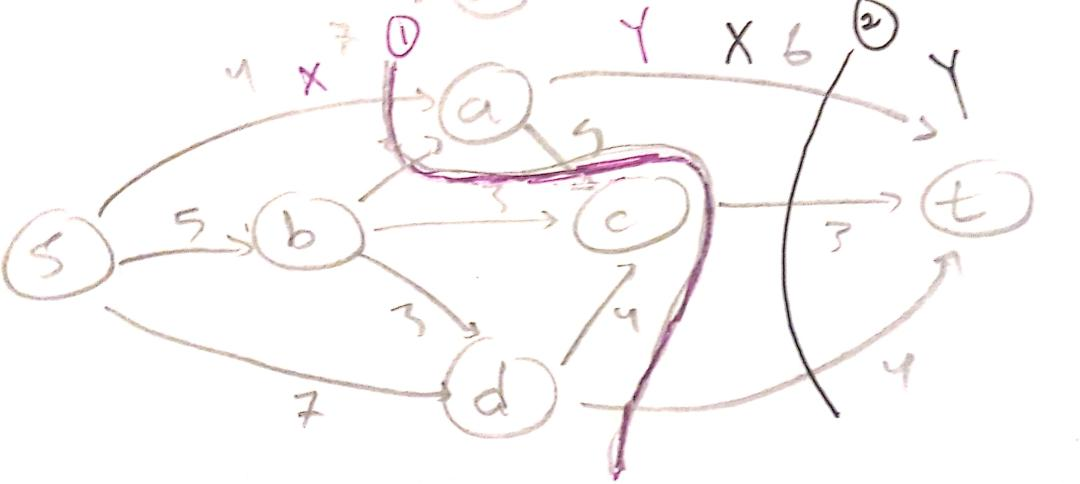
\includegraphics[width=\textwidth]{fig/5.jpg}
\caption*{Graph 5: the minimum cut for two cuts. \textit{Note: $b->a$ is 2 and $b->c$ is 3}

The purple line is for the $(\{s, b, c, d\},\{a, t\})$ maximum cut.

The black line for the $(\{s, a, b, c, d\},\{t\})$ maximum cut.}
\end{center}
\centering
\end{figure}


\end{document}
